\section{Prescribed ports on nonparallel cuts}\label{c:tilted}
The difference from the preceding two geometries is that a normal bridge
prefix changes the distance to the opposite support. Summing over that
support first gives an almost exhaustive prefix construction. We must
then show that its small exceptional mass stays small at a specified port.
All estimates below are uniform on a fixed compact set of the
nondegenerate wedge geometries in Theorem~\ref{c:main}. We continue to use
$d=\sqrt3/2$ and the winding spin $\sigma=3/8$.

\begin{theorem}[Tilted prescribed endpoints]\label{c:tilted-law}
In a pure wedge of angle $\pi/3$ or $2\pi/3$, take one prescribed port on each boundary ray. Suppose they have order-$R$ clearance to the opposite cut and distance $O(R)$
from the apex. Under the critical chord law their length is
$R^{4/3+o(1)}$ in probability. The conclusion persists after restriction
to the hexagons of Theorem~\ref{c:main} with the same side-interior
limiting data.
\end{theorem}
We now treat the case when the supporting sides at the two marked midpoints have distinct, nonparallel pure directions. Write \(W\) for the full wedge given by the two corresponding row cuts, and \(n,m\) for their inward unit normals in source and target order. Write \(a,Q\) for the midpoints. Both endpoints have clearance to the other cut of order \(R\), and their distances from the apex are \(O(R)\). We let \(R\to\infty\); constants may use fixed compact bounds on this nondegenerate scaled geometry. Until restricting the domain at the end we count paths in \(W\). Denote their mass at a specific endpoint \(U\) on the target ray by \(K(a,U;W)\) (abbreviated to \(K_U\)).



First we explain exhaustion by normal bridge prefixes when \emph{summing} over the target ray. Put \(r\) equal to the distance from \(a\) to the target support line in row-spacing units, and \(F(r)\) equal to \(\sum_U K_U\) along that ray. With directions fixed, the parameter alone determines this mass, by lattice translation (fix the start and its entire line); its possible values here are positive half-odd levels. This function decreases: keeping the source line fixed, the wedge expands as \(r\) increases, and the real contour identity gives
\[
 1=\cos(\sigma\pi) A(r)+\cos(\sigma\theta) F(r)
\]
where \(A\) sums exits back to the initial support, and \(\theta\) is the opening angle (\(\pi/3\) or \(2\pi/3\)). Indeed turns to the other side have magnitude \(\theta\); distant truncating exits vanish by the diameter bound. Thus monotonicity follows from that of \(A\). Also \(F(r)\lesssim(1+r)^{-1/4}\).



Use the ordinary iid irreducible pieces directed along \(n\). For each deterministic \(k\), call the prefix admissibly small when the sum of the \(k\) diameters \(J\) (enlarged by a constant if needed) is less than a sufficiently small fixed multiple of the source clearance to the other line. Write \(w\) for its displacement. Then
\[
 F(r)\ \ge\ \mathbb E[{\bf1}_{\rm small} F(r+m\cdot w/d)],
\]
by using the smaller wedge \(W'\) with initial support now passing through \(a'=a+w\), appending its chords at \(a'\). All points along the prefix avoid the target line. Weights multiply, and one recognizes the prefix by the first \(k\) positive single-crossing levels parallel to the initial support (the last one also separates the appended path strictly).



We record why \(F(r+o(r))-F(r)=o(r^{-1/4})\). For any large scale \(q\) there is \(k\le C q^{3/4}\) with probability bounded below of \(m\cdot w/d\le -b_0 q\) for some fixed \(b_0>0\). Indeed the source bridges of heights in \([q,2q]\) have summed mass \(\gtrsim q^{3/4}\) with such displacement, by Lemma~\ref{c:positive-projection} with second direction \(-m\). Equivalently use point-to-point corridors to macroscopic intervals on the top in a bounded range of slopes with that strict projection. Terms with more than \(C q^{3/4}\) pieces cost at most \(O(q^{3/4}e^{-c C})\) by the height Laplace deficit. This proves the assertion via renewal. At these orders \(k\), probability that the diameter sum exceeds \(Tq\) is \(O(T^{-3/4})\) for \(T\ge1\), by the tail bound and truncation.



If there is a drop at least \(\epsilon r^{-1/4}\) between \(r-l,r+l\) with \(1\le l=o(r)\) along a sequence (round levels throughout), choose a large fixed \(A_0\), then \(l\ll q\ll r\) with variation on \([r+b_0 q/4,r+(A_0+b_0+1)q]\) equal to \(o(r^{-1/4})\). Indeed one can test arbitrarily many disjoint such geometric bands and use monotonicity. Apply the inequality at \(j\) near \(r+b_0 q/2\) with the indicated \(k\). On small prefixes with \(|m\cdot w/d|\le A_0 q\) the joining factor is at least \(F(j)-o(r^{-1/4})\); if the shift is \(\le-b_0 q\) it gains at least \(\epsilon r^{-1/4}\). Smallness has probability tending to one; the remaining offset loss is arbitrarily small in probability by choice of \(A_0\). Since \(F(j)\lesssim r^{-1/4}\), this is impossible.



In particular take \(k=\lfloor R^{3/4-\eta}\rfloor\), fixed small \(\eta>0\). In the given geometries use a common smallness cutoff on \(\sum J\) at a sufficiently small fixed multiple of \(R\) (less than a small fraction of both endpoint clearances). Define exceptional paths to be all chords not so constructed with this prefix and a chord in \(W'\), and denote their mass at \(U\) by \(E_U\). By the last continuity, truncation and \(r\asymp R\), the constructed total in expectation over small prefixes differs from \(F(r)\) by \(o(R^{-1/4})\). Hence \(\sum_U E_U=o(R^{-1/4})\).



\subsection{Visits near the prescribed target}\label{c:tilted-visits}
The prefix construction has so far controlled only the sum of exceptional
masses. To pass to a single target, we need a bound for paths that approach
that target before ending a specified distance away. We give a local visit estimate. For \(q\le cR\), consider paths from \(a\) to points \(P\) on the target ray at distance between \(q\) and \(2q\) from \(Q\), also coming within \(t\) of \(Q\), \(1\le t\le q\). Their total mass satisfies
\begin{equation}\label{c:tilted-visit-bound}
 H_q(t)\ \lesssim\ R^{-1/4}(t/q)^{3/8}.
\end{equation}
Here and below \(c>0\) can be taken small relative to the compact geometry bounds. Use the fixed-source construction of Proposition~\ref{c:attachment-proposition}, with the side-1 outer landing exactly at \(a\) and side-2 outer landing free. Take translation scale a small fixed multiple of \(q\), so all bridge portions and translations have excursion less than (say) \(q/20\), with gaps between original and translated levels at each end of order \(q\). If \(q\) is bounded the estimate already follows from diameter. The first summed indicator mass is at least \(c_1 q^{1/2}H_q(t)\), using \(\gtrsim q^{3/4}\) summed bridge mass from \(a\) to its translates and \(\gtrsim q^{-1/4}\) on side 2. The target measure (paths from \(a\) to the other ray) has mass \(O(R^{-1/4})\).



For simultaneous translations \(v,v'\), split at both support crossings
on each branch in level order as in the chord construction. The orders
may differ at the two ends. All initial crossings still precede both
terminal crossings, by localization of the two exterior branches.
Write \(P_v,P_{v'}\) for the terminal ports of the two input chords;
each lies in the bin at distance between \(q\) and \(2q\) from \(Q\).
For \(t\le q/10\), a visit near either translated landmark \(Q+v\) or
\(Q+v'\) cannot lie on an exterior branch. The initial branches remain
at distance of order \(R\) from these landmarks. Each terminal branch
has excursion less than \(q/20\) from its endpoint \(P_v+v\) or
\(P_{v'}+v'\);
the endpoint bin and the small translation scale keep every such
endpoint at distance comparable to \(q\) from both landmarks.
Thus both visits occur after both initial crossings and before both
terminal crossings.

This common central portion stays above both target cuts. Its visit
within \(t\) of the landmark on the lower cut therefore forces
\(|m\cdot(v-v')|\le Ct\). Moreover, the chord between the innermost
cuts retains the visit to the landmark belonging to its own terminal
cut. Its terminal point is the translated \(P\) from that same list,
so its distance to the landmark is still in the prescribed bin; its
initial point is also prescribed. The endpoints and landmark have
only shifted by \(O(q)\), so this mixed-cut wedge has comparable compact
geometry bounds. If the visit estimate is known with exponent
\(\alpha\) for these geometries, its central mass is consequently at
most \(CR^{-1/4}(t/q)^\alpha\). The diameter bound starts this argument
at \(\alpha=0\).



The mixed difference factor now sums to \(O(t^{1/2})\):
\[
 \sum_{z:\ |m\cdot z|\le C t}D_n(z)(1+|m\cdot z|)^{-1/4}\le C' t^{1/2},
\]
with \(D_n\) defined before Lemma~\ref{c:mixed-displacement}. The
projected concentration and negative-quarter-moment bounds in
\eqref{c:projected-concentration} bound the contribution from \(j\)
pieces by
\(C\min(j^{-1/3},(1+t)^{3/4}j^{-4/3})\).
Summing in \(j\) by renewal, including ties, proves the restricted
estimate. The outer side-2 bridge costs \(O(q^{-1/4})\); the side-1
outer cost \(D_n(v_{\rm out})\) sums to \(O(q^{3/4})\), where
\(v_{\rm out}\) gives the side-1 outer crossing. Drop mutual avoidance
constraints between the difference, center and outer portions and
multiply their upper bounds. The summed second moment is at most
\[
 C q^{1/2}t^{1/2}\,R^{-1/4}(t/q)^\alpha .
\]
Cauchy--Schwarz proves the assertion with exponent \(1/4+\alpha/2\) (the remaining \(t\ge q/10\) always follows by diameter). Applying twice proves the displayed estimate; the shifts of supports in this finite bootstrap are \(O(q)\) each, so one can enlarge the compact bounds a little and decrease the allowed relative scale \(c\) at each step.



\subsection{An endpointwise comparison}\label{c:tilted-comparison}
We adapt the exterior-arc comparison from
\cite[proof of Proposition 7.1]{UniformMarked} to the nonparallel supports.
Take two individual endpoints \(P,Q\), with \(P\) nearer the apex and \(|P-Q|\in[q,2q]\). Add a formal connection from $P$ to $Q$ in the exterior of the target half-plane: a semicircle tangent to the normal rays at its anchors. This arc is not a honeycomb walk. Assign it modulus weight one, no visited-center length, and the phase $e^{i\sigma\Delta W}$ of its geometric turn. Sum only paths using the arc exactly once; all their other edges and vertex weights are ordinary. The arc's exterior lies outside $W$, so it meets no ordinary path away from its anchors. Figure~\ref{c:fig:arc} records its orientation. Arrange the coordinates so the initial ray points right, and the target ray lies counterclockwise at angle \(\theta\). Thus \(a\to P,a\to Q\) turn by \(\theta\); the arc \(P\to Q\) turns by \(-\pi\). For a path \(\omega:a\to Q\) define
\[
 f_W(P;\omega)=\frac1{2\cos(\sigma\pi)}-
 \sum_{b'\in(P,Q)}\ 
 \sum_{\substack{\zeta:P\to b'\ \text{in }W\\ \zeta\text{ disjoint from }\omega}}
 \kappa^{L(\zeta)}.
\]
For paths to \(P\) use \(f_W(Q;\omega)\) analogously with continuation from \(Q\) and the same open interval. Then (integrals denoting critical weighted sums)
\[
 \left|\int_{a\to Q} f_W(P;\omega)-\int_{a\to P} f_W(Q;\omega)\right|
 \le C R^{-1/4}(K_Q+K_P).
\]
Indeed the flux delivered by arc traversals before further continuation equals the outgoing flux using the arc once. Prefix cancellations at all ordinary vertices preserve the count of arc uses under unfinished-loop reversal; the whole arc is well after the initial cut so the source cannot be inside a loop. Use first a large convex truncation; distant contributions vanish by ordinary diameter bounds. After rotation by \(e^{-i\sigma\theta}\) the imaginary input is \(\sin(\sigma\pi)(K_Q-K_P)\). Outputs back to the initial support have modulus cost at most \(C R^{-1/4}(K_Q+K_P)\). Outputs on the target support from an initial traversal \(a\to Q\), then the arc to \(P\), must end nearer than \(Q\) by noncrossing. If ending even before \(P\) their relative phase after rotation is 1, while in the open interval it has imaginary part \(\sin(2\sigma\pi)\) (final arch positive turn \(\pi\)). Similarly from \(a\to P\) the only target-side terms with imaginary part end in \((P,Q)\), with opposite sign. Neither anchor can be such a final exit (used triangles). Dividing by \(\sin(2\sigma\pi)\) proves the comparison.



Reflection and the half-plane contour identity give total arch mass
\(1/(2\cos(\sigma\pi))\) in each direction. Together with the
half-plane arch estimates, this gives, for paths to \(Q\),
\begin{equation}\label{c:tilted-completion-bounds}
 c' q^{-1/4}\le f_W(P;\omega)\le C(1+\min(q,\operatorname{dist}(P,\omega)))^{-1/4}
\end{equation}
and analogously after exchanging the endpoints. Indeed all completions counted there are among half-plane arches in one direction, but omitting at least the long-offset tail of mass \(\gtrsim q^{-1/4}\). All sufficiently small diameter ones up to scale the indicated minimum are included, by clearance and disjointness, and the diameter tail bounds the loss.



With \(q\) a sufficiently small fixed fraction of \(R\), the comparison absorbs the \(O(R^{-1/4})K_Q\) term. On the other side average over the order \(q\) choices of \(P\). The visit bound \(H_q(t)\), with exponent \(>1/4\), pays for the upper estimate on \(f_W(Q;\omega)\) by dyadic summation. More explicitly the total over \(P\) of these upper integrals costs \(O(R^{-1/4}q^{-1/4})\), including unit and smaller distances and also paths always at distance \(>q\). This yields the uniform bound \(K_Q\lesssim R^{-5/4}\).




\begin{figure}[htbp]
\centering
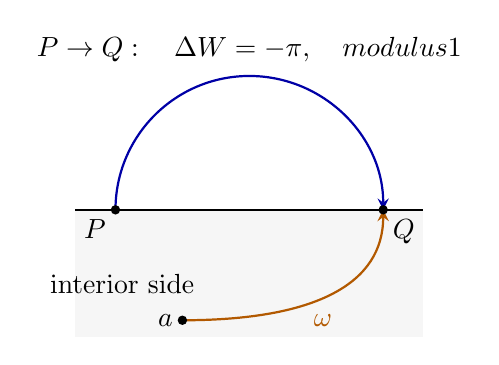
\begin{tikzpicture}[scale=.85,>=stealth]
 \fill[gray!7] (-.6,-1.9) rectangle (4.6,0);
 \draw[thick] (-.6,0)--(4.6,0);
 \draw[blue!65!black,thick,->] (0,0) arc[start angle=180,end angle=0,radius=2];
 \draw[orange!70!black,thick,->] (1,-1.65) .. controls (3,-1.65) and (4,-1.1) .. (4,0);
 \fill (0,0) circle(2pt) node[below left] {$P$};
 \fill (4,0) circle(2pt) node[below right] {$Q$};
 \fill (1,-1.65) circle(2pt) node[left] {$a$};
 \node at (2,2.4) {$P\to Q:\quad\Delta W=-\pi,\quad\text{modulus }1$};
 \node[orange!70!black] at (3.1,-1.65) {$\omega$};
 \node at (.1,-1.1) {interior side};
\end{tikzpicture}
\caption{Local orientation at the target support, rotated to horizontal.
The blue semicircle is a formal exterior connection, not an added lattice
path. The orange path arrives at $Q$ from the interior; its continuation
through the arc uses the reverse orientation. The schematic suppresses
the source support and the lattice.}\label{c:fig:arc}
\end{figure}

\subsection{Removing the exceptional mass}\label{c:tilted-exceptional}
The bound for each individual kernel is now available. Apply the same
comparison to the exceptional set left by the prefix construction.
The same absolute comparison holds with the two left integrals restricted to exceptional paths and the right error still \(C R^{-1/4}(K_Q+K_P)\), with \(C\) independent of \(q\le cR\). To see this, subtract the comparison (in signed-difference form with its error) in \(W'\), starting at \(a'\), integrated over small prefixes. Its right error costs at most the same amount by the prefix injection. And the difference of the two \(f\) factors for a central path and full constructed path costs only \(O(R^{-1/4})\) each, since central completions in the sum stay beyond the prefix cut and avoid the prefix too, and any discarded full-domain completions must reach that cut from clearance of order \(R\). The constants are uniform by smallness of the prefixes.



Fix \(q\) of order \(\rho R\) for small fixed \(\rho>0\), and put
\[
 e_R=R^{1/4}\sum_U E_U\longrightarrow0.
\]
Let \(I_R(q)\) be the sum over the order-\(q\) choices of \(P\) of
\(\int_{a\to P,\,\mathrm{exceptional}}f_W(Q;\omega)\).
To control its possibly singular weight, fix \(0<\delta<1/2\).
Paths with \(\operatorname{dist}(Q,\omega)\ge\delta q\) contribute at
most \(C(\delta q)^{-1/4}\sum_P E_P\), by
\eqref{c:tilted-completion-bounds}. For the remaining paths, discard
the exceptional restriction and sum
\eqref{c:tilted-visit-bound} over dyadic distance bins below \(\delta q\).
The exponent \(3/8-1/4=1/8\) is positive, so, including the final
bounded-distance bin, for \(R\) sufficiently large at fixed
\(\rho,\delta\) this gives
\[
 I_R(q)\le C R^{-1/4}q^{-1/4}
       \bigl(\delta^{-1/4}e_R+\delta^{1/8}\bigr).
\]
First let \(R\to\infty\) at fixed \(\rho,\delta\), then let
\(\delta\downarrow0\). Thus \(I_R(q)=o(R^{-1/4}q^{-1/4})\) for
each fixed \(\rho\). Averaging the exceptional comparison over its
order-\(q\) ports, using the lower bound in
\eqref{c:tilted-completion-bounds} and the individual kernel upper
bound, now yields
\[
 q^{-1/4} E_Q \le o(R^{-1/4}q^{-5/4})+C R^{-1/4} R^{-5/4}.
\]
Here the little-oh may depend on \(\rho\), but the comparison error
constant \(C\) does not. In particular
\[
 \limsup_{R\to\infty}R^{5/4}E_Q\le C\rho^{1/4}.
\]
Letting \(\rho\downarrow0\) proves \(E_Q=o(R^{-5/4})\).



\subsection{The prescribed length law}
Finally count lengths violating either power bound
\(R^{4/3\pm\epsilon}\). Up to mass \(o(R^{-5/4})\), the prefix
construction applies at the prescribed \(Q\). Under the iid law its
prefix length has exponent
\[
 \frac{3/4-\eta}{9/16}=\frac43-\frac{16\eta}{9}
\]
in probability. On small prefixes the center factor is at most
\(CR^{-5/4}\), uniformly in their displacements. Therefore an iid
event of probability \(o(1)\) contributes constructed mass
\(o(R^{-5/4})\), without asserting independence after fixing \(Q\).
Choose \(\eta<9\epsilon/16\). This proves the short-length bound
and also makes prefixes longer than \(\frac12R^{4/3+\epsilon}\)
negligible.

For the appended chord, any specific prefix displacement costs
\(O(k^{-8/3})\) by Proposition~\ref{c:planar-atoms}. Align all new
wedges by lattice translations \(\tau_w\); their apex intersections
are triangular lattice vertices. In the common wedge the endpoints are
\[
 x_w=a+w+\tau_w,\qquad y_w=Q+\tau_w,
 \qquad w=(x_w-y_w)-(a-Q).
\]
Thus each endpoint pair determines its prefix displacement. Since the
angles are fixed and \(|w|=O(R)\) for small prefixes, the apex shift
\(\tau_w\) is also \(O(R)\). In particular there are only \(O(R)\)
possible aligned source ports, all at distance \(O(R)\) from the apex.

We may now sum freely over the endpoint pairs. For appended chords
of diameter above \(S_*=R^{1+\lambda}\), the one-source diameter
bound and the number of sources give \(CRS_*^{-1/4}\).
All smaller-diameter chords lie in a common convex pure truncation of
diameter \(O(S_*)\). The all-endpoint length-mass bound there shows
that those of length above \(\frac12R^{4/3+\epsilon}\) have total mass
at most \(CR^{-4/3-\epsilon}S_*^{25/12+o(1)}\).
Multiplying these two estimates by \(k^{-8/3}\), respectively, gives
\[
 CR^{-5/4-\lambda/4+8\eta/3},\qquad
 R^{-5/4-\epsilon+25\lambda/12+8\eta/3+o(1)}.
\]
Choose first \(\lambda>0\) so that \(25\lambda/12<\epsilon\), then
\(\eta>0\) sufficiently small that both exponents are strictly below
\(-5/4\), while retaining \(\eta<9\epsilon/16\). Both appended-chord
exceptions are consequently \(o(R^{-5/4})\).



Restriction to a hexagon in Theorem~\ref{c:main} can only decrease
these absolute exceptional masses. Its own normalizer is at least
\(cR^{-5/4}\), by Proposition~\ref{c:connectors} and the endpoint
clearances. Dividing proves that both tails vanish in probability
in the restricted domain as well as in the full wedge.

This proves Theorem~\ref{c:tilted-law}. Together with
Theorem~\ref{c:same-side-law} and Theorem~\ref{c:parallel}, it proves
Theorem~\ref{c:main}: the two side supports are identical, parallel, or
nonparallel, and the connector lower bound supplies the normalizer in
each finite hexagon.
